% Options for packages loaded elsewhere
\PassOptionsToPackage{unicode}{hyperref}
\PassOptionsToPackage{hyphens}{url}
%
\documentclass[
]{book}
\title{Robustheit und Voraussetzungstests}
\author{Max Brede und Johannes Andres}
\date{2021-10-05}

\usepackage{amsmath,amssymb}
\usepackage{lmodern}
\usepackage{iftex}
\ifPDFTeX
  \usepackage[T1]{fontenc}
  \usepackage[utf8]{inputenc}
  \usepackage{textcomp} % provide euro and other symbols
\else % if luatex or xetex
  \usepackage{unicode-math}
  \defaultfontfeatures{Scale=MatchLowercase}
  \defaultfontfeatures[\rmfamily]{Ligatures=TeX,Scale=1}
\fi
% Use upquote if available, for straight quotes in verbatim environments
\IfFileExists{upquote.sty}{\usepackage{upquote}}{}
\IfFileExists{microtype.sty}{% use microtype if available
  \usepackage[]{microtype}
  \UseMicrotypeSet[protrusion]{basicmath} % disable protrusion for tt fonts
}{}
\makeatletter
\@ifundefined{KOMAClassName}{% if non-KOMA class
  \IfFileExists{parskip.sty}{%
    \usepackage{parskip}
  }{% else
    \setlength{\parindent}{0pt}
    \setlength{\parskip}{6pt plus 2pt minus 1pt}}
}{% if KOMA class
  \KOMAoptions{parskip=half}}
\makeatother
\usepackage{xcolor}
\IfFileExists{xurl.sty}{\usepackage{xurl}}{} % add URL line breaks if available
\IfFileExists{bookmark.sty}{\usepackage{bookmark}}{\usepackage{hyperref}}
\hypersetup{
  pdftitle={Robustheit und Voraussetzungstests},
  pdfauthor={Max Brede und Johannes Andres},
  hidelinks,
  pdfcreator={LaTeX via pandoc}}
\urlstyle{same} % disable monospaced font for URLs
\usepackage{color}
\usepackage{fancyvrb}
\newcommand{\VerbBar}{|}
\newcommand{\VERB}{\Verb[commandchars=\\\{\}]}
\DefineVerbatimEnvironment{Highlighting}{Verbatim}{commandchars=\\\{\}}
% Add ',fontsize=\small' for more characters per line
\usepackage{framed}
\definecolor{shadecolor}{RGB}{248,248,248}
\newenvironment{Shaded}{\begin{snugshade}}{\end{snugshade}}
\newcommand{\AlertTok}[1]{\textcolor[rgb]{0.94,0.16,0.16}{#1}}
\newcommand{\AnnotationTok}[1]{\textcolor[rgb]{0.56,0.35,0.01}{\textbf{\textit{#1}}}}
\newcommand{\AttributeTok}[1]{\textcolor[rgb]{0.77,0.63,0.00}{#1}}
\newcommand{\BaseNTok}[1]{\textcolor[rgb]{0.00,0.00,0.81}{#1}}
\newcommand{\BuiltInTok}[1]{#1}
\newcommand{\CharTok}[1]{\textcolor[rgb]{0.31,0.60,0.02}{#1}}
\newcommand{\CommentTok}[1]{\textcolor[rgb]{0.56,0.35,0.01}{\textit{#1}}}
\newcommand{\CommentVarTok}[1]{\textcolor[rgb]{0.56,0.35,0.01}{\textbf{\textit{#1}}}}
\newcommand{\ConstantTok}[1]{\textcolor[rgb]{0.00,0.00,0.00}{#1}}
\newcommand{\ControlFlowTok}[1]{\textcolor[rgb]{0.13,0.29,0.53}{\textbf{#1}}}
\newcommand{\DataTypeTok}[1]{\textcolor[rgb]{0.13,0.29,0.53}{#1}}
\newcommand{\DecValTok}[1]{\textcolor[rgb]{0.00,0.00,0.81}{#1}}
\newcommand{\DocumentationTok}[1]{\textcolor[rgb]{0.56,0.35,0.01}{\textbf{\textit{#1}}}}
\newcommand{\ErrorTok}[1]{\textcolor[rgb]{0.64,0.00,0.00}{\textbf{#1}}}
\newcommand{\ExtensionTok}[1]{#1}
\newcommand{\FloatTok}[1]{\textcolor[rgb]{0.00,0.00,0.81}{#1}}
\newcommand{\FunctionTok}[1]{\textcolor[rgb]{0.00,0.00,0.00}{#1}}
\newcommand{\ImportTok}[1]{#1}
\newcommand{\InformationTok}[1]{\textcolor[rgb]{0.56,0.35,0.01}{\textbf{\textit{#1}}}}
\newcommand{\KeywordTok}[1]{\textcolor[rgb]{0.13,0.29,0.53}{\textbf{#1}}}
\newcommand{\NormalTok}[1]{#1}
\newcommand{\OperatorTok}[1]{\textcolor[rgb]{0.81,0.36,0.00}{\textbf{#1}}}
\newcommand{\OtherTok}[1]{\textcolor[rgb]{0.56,0.35,0.01}{#1}}
\newcommand{\PreprocessorTok}[1]{\textcolor[rgb]{0.56,0.35,0.01}{\textit{#1}}}
\newcommand{\RegionMarkerTok}[1]{#1}
\newcommand{\SpecialCharTok}[1]{\textcolor[rgb]{0.00,0.00,0.00}{#1}}
\newcommand{\SpecialStringTok}[1]{\textcolor[rgb]{0.31,0.60,0.02}{#1}}
\newcommand{\StringTok}[1]{\textcolor[rgb]{0.31,0.60,0.02}{#1}}
\newcommand{\VariableTok}[1]{\textcolor[rgb]{0.00,0.00,0.00}{#1}}
\newcommand{\VerbatimStringTok}[1]{\textcolor[rgb]{0.31,0.60,0.02}{#1}}
\newcommand{\WarningTok}[1]{\textcolor[rgb]{0.56,0.35,0.01}{\textbf{\textit{#1}}}}
\usepackage{longtable,booktabs,array}
\usepackage{calc} % for calculating minipage widths
% Correct order of tables after \paragraph or \subparagraph
\usepackage{etoolbox}
\makeatletter
\patchcmd\longtable{\par}{\if@noskipsec\mbox{}\fi\par}{}{}
\makeatother
% Allow footnotes in longtable head/foot
\IfFileExists{footnotehyper.sty}{\usepackage{footnotehyper}}{\usepackage{footnote}}
\makesavenoteenv{longtable}
\usepackage{graphicx}
\makeatletter
\def\maxwidth{\ifdim\Gin@nat@width>\linewidth\linewidth\else\Gin@nat@width\fi}
\def\maxheight{\ifdim\Gin@nat@height>\textheight\textheight\else\Gin@nat@height\fi}
\makeatother
% Scale images if necessary, so that they will not overflow the page
% margins by default, and it is still possible to overwrite the defaults
% using explicit options in \includegraphics[width, height, ...]{}
\setkeys{Gin}{width=\maxwidth,height=\maxheight,keepaspectratio}
% Set default figure placement to htbp
\makeatletter
\def\fps@figure{htbp}
\makeatother
\setlength{\emergencystretch}{3em} % prevent overfull lines
\providecommand{\tightlist}{%
  \setlength{\itemsep}{0pt}\setlength{\parskip}{0pt}}
\setcounter{secnumdepth}{5}
\usepackage{booktabs}
\usepackage{tikz}

\newenvironment{cols}[1][]{}{}

\newenvironment{col}[1]{\begin{minipage}{#1}\ignorespaces}{%
\end{minipage}
\ifhmode\unskip\fi
\aftergroup\useignorespacesandallpars}

\def\useignorespacesandallpars#1\ignorespaces\fi{%
#1\fi\ignorespacesandallpars}

\makeatletter
\def\ignorespacesandallpars{%
  \@ifnextchar\par
    {\expandafter\ignorespacesandallpars\@gobble}%
    {}%
}
\makeatother

\usetikzlibrary{arrows, arrows.meta, calc, positioning, quotes, shapes}
\tikzset{
    mynode/.style={draw,text width=1in,align=center},
    mylabel/.style={text width=7em}
}

\definecolor{White}{gray}{1}
\definecolor{Black}{gray}{0}
\definecolor{Gray}{gray}{0.5}
\definecolor{LightGray}{gray}{0.99}
\definecolor{DarkGray}{gray}{0.6}
\definecolor{LightBlue}{rgb}{0.9 0.9 1}
\definecolor{Blue}{rgb}{0.55 0.55 1}
\definecolor{DarkBlue}{rgb}{0.2 0.2 1}
\definecolor{Red}{rgb}{1 0 0}
\definecolor{DarkRed}{rgb}{0.7 0 0}
\definecolor{Green}{rgb}{0 0.8 0.2}


\usepackage{lscape}
\newcommand{\blandscape}{\begin{landscape}}
\newcommand{\elandscape}{\end{landscape}}
\usepackage{booktabs}
\usepackage{longtable}
\usepackage{array}
\usepackage{multirow}
\usepackage{wrapfig}
\usepackage{float}
\usepackage{colortbl}
\usepackage{pdflscape}
\usepackage{tabu}
\usepackage{threeparttable}
\usepackage{threeparttablex}
\usepackage[normalem]{ulem}
\usepackage{makecell}
\usepackage{xcolor}
\ifLuaTeX
  \usepackage{selnolig}  % disable illegal ligatures
\fi
\usepackage[]{natbib}
\bibliographystyle{apalike}

\begin{document}
\maketitle

{
\setcounter{tocdepth}{1}
\tableofcontents
}
\hypertarget{vorwort}{%
\chapter{Vorwort}\label{vorwort}}

Dieses mit \texttt{bookdown} erstellte Dokument ist das Skript zum Seminar ``psyM9-1: Psychologische Forschungsmethoden. Projektseminar I'' und ``PSY\_B\_20\_e-1: Forschungsorientierte Vertiefung: Forschungsmethoden'' der CAU zu Kiel.

\hypertarget{lehrplan}{%
\chapter{Lehrplan}\label{lehrplan}}

\hypertarget{semesterplan}{%
\section{Semesterplan}\label{semesterplan}}

\blandscape
\scriptsize

\begin{longtable}[t]{>{\raggedright\arraybackslash}p{0.33in}>{\raggedright\arraybackslash}p{0.4in}>{\raggedright\arraybackslash}p{0.7in}>{\raggedright\arraybackslash}p{1.5in}>{}p{2.5in}>{}p{0.75in}}
\toprule
Sitzung & Datum & Sitzungstitel & Lernziele\\
\midrule
 &  &  & Die Studierenden…\\
1 & 2021-10-25 & Rste Codeschnipsel & können Funktionen in R definieren, deren Bestandteile nennen und diese benutzen.\\
 &  &  & wissen, was if-Statements sind und können diese in R einsetzen\\
2 & 2021-11-01 & Iterationen und Zufallszahlen & wissen, was for- und while-Schleifen sind und können diese in R einsetzen\\
 &  &  & können Werte von Zufallszahlen in R erzeugen\\
\addlinespace
3 & 2021-11-08 & Listen und Matrizen & wissen, wie eine „list“ in R aufgebaut ist und können diese benutzen\\
 &  &  & können Matrizen in R benutzen\\
4 & 2021-11-15 & Welche Iterationen? & kennen verschiedene Arten von Rs iterativen „functionals“ und können diese benutzen\\
 &  &  & können basales microbenchmarking einsetzen um Funktionsperformance zu evaluieren\\
5 & 2021-11-22 & Erste Simulation I & können geschachtelte Schleifen und iterative functionals nutzen\\
\addlinespace
6 & 2021-11-29 & Erste Simulation II & \\
7 & 2021-12-06 & Beispiele & \\
8 & 2021-12-13 & Beispiele & \\
9 & 2021-12-20 &  & \\
10 & 2022-01-10 &  & \\
\addlinespace
11 & 2022-01-17 &  & \\
12 & 2022-01-24 &  & \\
13 & 2022-01-31 &  & \\
14 & 2022-02-07 &  & \\
15 & 2022-02-14 &  & \\
\bottomrule
\end{longtable}
\normalsize
\elandscape
\newpage

\hypertarget{programmieren-in-r}{%
\chapter{Programmieren in R}\label{programmieren-in-r}}

\hypertarget{funktionen}{%
\section{Funktionen}\label{funktionen}}

Wir kennen Funktionen ja schon aus den EDV-Veranstaltungen.

Zum Beispiel macht die \texttt{sum}-Funktion mit einem Vektor das, was der Name sagt:

\begin{Shaded}
\begin{Highlighting}[]
\FunctionTok{sum}\NormalTok{(}\FunctionTok{c}\NormalTok{(}\DecValTok{1}\NormalTok{,}\DecValTok{2}\NormalTok{,}\DecValTok{3}\NormalTok{))}
\end{Highlighting}
\end{Shaded}

\begin{verbatim}
## [1] 6
\end{verbatim}

\begin{Shaded}
\begin{Highlighting}[]
\DecValTok{1} \SpecialCharTok{+} \DecValTok{2} \SpecialCharTok{+} \DecValTok{3}
\end{Highlighting}
\end{Shaded}

\begin{verbatim}
## [1] 6
\end{verbatim}

Funktionen können wir auch selbst definieren. Eine Funktion, die uns begrüßt könnte zum Beispiel wie folgt aussehen:

\begin{Shaded}
\begin{Highlighting}[]
\NormalTok{greet\_me }\OtherTok{\textless{}{-}} \ControlFlowTok{function}\NormalTok{()\{}
  \FunctionTok{return}\NormalTok{(}\StringTok{\textquotesingle{}Hello! Nice to see you!\textquotesingle{}}\NormalTok{)}
\NormalTok{\}}
\end{Highlighting}
\end{Shaded}

Wenn wir jetzt die \texttt{greet\_me}-Funktion aufrufen, sehen wir:

\begin{Shaded}
\begin{Highlighting}[]
\FunctionTok{greet\_me}\NormalTok{()}
\end{Highlighting}
\end{Shaded}

\begin{verbatim}
## [1] "Hello! Nice to see you!"
\end{verbatim}

In der Funktionsdefinition können wir ein paar Teile wiederkennen.
Zum Einen ist da der \texttt{greet\_me\ \textless{}-}-Teil, den wir ja schon als Objektzuweisung kennen. Wir weisen also dem Ergebnis eines Ausdrucks den Namen \texttt{greet\_me} zu.

Funktions-\emph{Objekte} werden also genauso wie Datensätze und Vektoren als eine Kombination von Namen und zugehörigem Inhalt definiert.

Dabei erstellt die Funktion \texttt{function()} einen Objektinhalt, der aus \emph{body} und \emph{formals} besteht und in einem \emph{environment} definiert ist.

Der \emph{body} ist der Teil der Funktion, der definiert, was passieren soll und wird in R in geschweiften Klammern hinter der \texttt{function}-Funktion definiert
In unserem Beispiel besteht der body aus dem Aufruf, einen Text zurückzugeben:

\begin{Shaded}
\begin{Highlighting}[]
\FunctionTok{body}\NormalTok{(greet\_me)}
\end{Highlighting}
\end{Shaded}

\begin{verbatim}
## {
##     return("Hello! Nice to see you!")
## }
\end{verbatim}

Die \emph{formals} sind die Argumente, die bei der Ausführung des \emph{body}s genutzt werden sollen.

In unserem Beispiel haben wir noch keine Argumente berücksichtigt:

\begin{Shaded}
\begin{Highlighting}[]
\FunctionTok{formals}\NormalTok{(greet\_me)}
\end{Highlighting}
\end{Shaded}

\begin{verbatim}
## NULL
\end{verbatim}

Wir könnten die Funktion aber neu definieren, so dass sie einen gegebenen Namen begrüßt. Dafür geben wir der \texttt{function}-Funktion ein Argument, das der Name des erwarteten Arguments sein soll:

\begin{Shaded}
\begin{Highlighting}[]
\NormalTok{greet\_someone }\OtherTok{\textless{}{-}} \ControlFlowTok{function}\NormalTok{(name)\{}
  \FunctionTok{return}\NormalTok{(}\FunctionTok{paste0}\NormalTok{(}\StringTok{\textquotesingle{}Hello \textquotesingle{}}\NormalTok{,name,}\StringTok{\textquotesingle{}! Nice to see you!\textquotesingle{}}\NormalTok{))}
\NormalTok{\}}

\FunctionTok{greet\_someone}\NormalTok{(}\StringTok{\textquotesingle{}Marvin\textquotesingle{}}\NormalTok{)}
\end{Highlighting}
\end{Shaded}

\begin{verbatim}
## [1] "Hello Marvin! Nice to see you!"
\end{verbatim}

Wenn wir uns jetzt nochmal die \texttt{formals} ausgeben lassen, sehen wir, dass ein Argument vorgesehen ist:

\begin{Shaded}
\begin{Highlighting}[]
\FunctionTok{formals}\NormalTok{(greet\_someone)}
\end{Highlighting}
\end{Shaded}

\begin{verbatim}
## $name
\end{verbatim}

Der letzte Teil einer Funktionsdefinition ist das \emph{environment}. Damit ist der Namensraum gemeint, auf den die Funktion zugreifen kann:

\begin{Shaded}
\begin{Highlighting}[]
\FunctionTok{environment}\NormalTok{(greet\_someone)}
\end{Highlighting}
\end{Shaded}

\begin{verbatim}
## <environment: R_GlobalEnv>
\end{verbatim}

In unserem Beispiel wurde die Funktion in der laufenden R-Session definiert (wie die allermeisten Funktionen, die wir dieses Semester nutzen werden). Der Output \texttt{R\_GlobalEnv} heißt also, dass die Funktion auf Objekte in der Haupt-R-Session zurückgreifen kann.

Praktisch heißt das, dass wir zum Beispiel Konstanten einmal außerhalb einer Funktion definieren können, die diese dann nutzen kann:

\begin{Shaded}
\begin{Highlighting}[]
\NormalTok{n }\OtherTok{\textless{}{-}} \DecValTok{10}

\NormalTok{greet\_someone\_n\_times }\OtherTok{\textless{}{-}} \ControlFlowTok{function}\NormalTok{(name) \{}
  \FunctionTok{return}\NormalTok{(}\FunctionTok{rep}\NormalTok{(}\FunctionTok{paste0}\NormalTok{(}\StringTok{\textquotesingle{}Hello \textquotesingle{}}\NormalTok{, }
\NormalTok{                    name, }
                    \StringTok{\textquotesingle{}! Nice to see you!\textquotesingle{}}\NormalTok{), }
\NormalTok{             n))}
\NormalTok{\}}

\FunctionTok{greet\_someone\_n\_times}\NormalTok{(}\StringTok{\textquotesingle{}Marvin\textquotesingle{}}\NormalTok{)}
\end{Highlighting}
\end{Shaded}

\begin{verbatim}
##  [1] "Hello Marvin! Nice to see you!" "Hello Marvin! Nice to see you!"
##  [3] "Hello Marvin! Nice to see you!" "Hello Marvin! Nice to see you!"
##  [5] "Hello Marvin! Nice to see you!" "Hello Marvin! Nice to see you!"
##  [7] "Hello Marvin! Nice to see you!" "Hello Marvin! Nice to see you!"
##  [9] "Hello Marvin! Nice to see you!" "Hello Marvin! Nice to see you!"
\end{verbatim}

Was das aber nicht heißt ist, dass die Funktion eine externe Variable ändern kann:

\begin{Shaded}
\begin{Highlighting}[]
\NormalTok{greet\_someone\_n\_times }\OtherTok{\textless{}{-}} \ControlFlowTok{function}\NormalTok{(name) \{}
  
\NormalTok{  n }\OtherTok{\textless{}{-}} \DecValTok{3}
  
  \FunctionTok{return}\NormalTok{(}\FunctionTok{rep}\NormalTok{(}\FunctionTok{paste0}\NormalTok{(}\StringTok{\textquotesingle{}Hello \textquotesingle{}}\NormalTok{, }
\NormalTok{                    name, }
                    \StringTok{\textquotesingle{}! Nice to see you!\textquotesingle{}}\NormalTok{), }
\NormalTok{             n))}
\NormalTok{\}}

\FunctionTok{greet\_someone\_n\_times}\NormalTok{(}\StringTok{\textquotesingle{}Marvin\textquotesingle{}}\NormalTok{)}
\end{Highlighting}
\end{Shaded}

\begin{verbatim}
## [1] "Hello Marvin! Nice to see you!" "Hello Marvin! Nice to see you!"
## [3] "Hello Marvin! Nice to see you!"
\end{verbatim}

\begin{Shaded}
\begin{Highlighting}[]
\NormalTok{n}
\end{Highlighting}
\end{Shaded}

\begin{verbatim}
## [1] 10
\end{verbatim}

Das liegt daran, dass die Funktion beim Aufrufen eine Kopie des globalen Environments als eigene Variablenumgebung zugewiesen bekommt und diese Kopie auch verändern kann. Die Kopie wird aber bei Beenden der Funktion verworfen, so dass Änderungen in der Funktion nicht erhalten bleiben.

Dabei werden die Argumente der Funktion dem Environment der Funktion hinzugefügt, wobei im Zweifelsfall gleichnamige Objekte für die Funktion überschrieben werden:

\begin{Shaded}
\begin{Highlighting}[]
\NormalTok{x }\OtherTok{\textless{}{-}} \DecValTok{1}\SpecialCharTok{:}\DecValTok{10}
\NormalTok{y }\OtherTok{\textless{}{-}} \DecValTok{11}\SpecialCharTok{:}\DecValTok{20}

\NormalTok{my\_function }\OtherTok{\textless{}{-}} \ControlFlowTok{function}\NormalTok{(x,y)\{}
  \FunctionTok{return}\NormalTok{(}\FunctionTok{c}\NormalTok{(x,y))}
\NormalTok{\}}

\FunctionTok{my\_function}\NormalTok{(}\DecValTok{21}\NormalTok{,}\DecValTok{22}\NormalTok{)}
\end{Highlighting}
\end{Shaded}

\begin{verbatim}
## [1] 21 22
\end{verbatim}

\hypertarget{aufgabe}{%
\subsection{Aufgabe}\label{aufgabe}}

\begin{enumerate}
\def\labelenumi{\arabic{enumi}.}
\item
  Erstelle eine Funktion mit dem Namen \texttt{my\_mean}, die den Mittelwert eines gegebenen Vektors berechnet.
\item
  Was ergibt der folgende Aufruf:
\end{enumerate}

\begin{Shaded}
\begin{Highlighting}[]
\NormalTok{dummy\_function }\OtherTok{\textless{}{-}} \ControlFlowTok{function}\NormalTok{(a,b)\{}
\NormalTok{  a }\SpecialCharTok{*}\NormalTok{ b}
\NormalTok{\}}

\NormalTok{c }\OtherTok{\textless{}{-}} \FunctionTok{dummy\_function}\NormalTok{(}\DecValTok{1}\NormalTok{,}\DecValTok{2}\NormalTok{)}

\FunctionTok{formals}\NormalTok{(dummy\_function)}
\end{Highlighting}
\end{Shaded}

\begin{enumerate}
\def\labelenumi{\arabic{enumi}.}
\setcounter{enumi}{2}
\tightlist
\item
  Was ist am Ende des folgenden Aufrufs in \texttt{number} abgelegt?
\end{enumerate}

\begin{Shaded}
\begin{Highlighting}[]
\NormalTok{number }\OtherTok{\textless{}{-}} \StringTok{\textquotesingle{}a number\textquotesingle{}}

\NormalTok{important\_calculation }\OtherTok{\textless{}{-}} \ControlFlowTok{function}\NormalTok{(number)\{}
\NormalTok{  number }\OtherTok{\textless{}{-}} \DecValTok{42} \SpecialCharTok{/}\NormalTok{ number }\SpecialCharTok{*}\NormalTok{ number}
  \FunctionTok{return}\NormalTok{(number)}
\NormalTok{\}}

\FunctionTok{important\_calculation}\NormalTok{(}\DecValTok{5}\NormalTok{)}
\end{Highlighting}
\end{Shaded}

\begin{verbatim}
## [1] 42
\end{verbatim}

Antworten

\textbf{1.}

\begin{Shaded}
\begin{Highlighting}[]
\NormalTok{my\_mean }\OtherTok{\textless{}{-}} \ControlFlowTok{function}\NormalTok{(x)\{}
  \FunctionTok{return}\NormalTok{(}\FunctionTok{sum}\NormalTok{(x)}\SpecialCharTok{/}\FunctionTok{length}\NormalTok{(x))}
\NormalTok{\}}
\end{Highlighting}
\end{Shaded}

\textbf{2.}

\begin{verbatim}
## $a
## 
## 
## $b
\end{verbatim}

\textbf{3.}

\texttt{\textquotesingle{}a\ number\textquotesingle{}}

\hypertarget{geschachtelte-funktionen}{%
\section{Geschachtelte Funktionen}\label{geschachtelte-funktionen}}

Um den Code übersichtlicher zu halten, können Teile von Funktionen in andere Funktionen ausgegliedert werden.
Dabei nutzen wir, dass unsere Funktionen auch auf das global Environment zugreifen und Funktionen ja auch nur Arten von Objekten sind.

Wenn wir unsere Funktionen \texttt{greet\_someone} und \texttt{greet\_someone\_n\_times} von vorhin nochmal angucken sehen wir, dass ein Teil des Codes in beiden auftaucht:

\begin{Shaded}
\begin{Highlighting}[]
\FunctionTok{print}\NormalTok{(greet\_someone)}
\end{Highlighting}
\end{Shaded}

\begin{verbatim}
## function(name){
##   return(paste0('Hello ',name,'! Nice to see you!'))
## }
\end{verbatim}

\begin{Shaded}
\begin{Highlighting}[]
\FunctionTok{print}\NormalTok{(greet\_someone\_n\_times)}
\end{Highlighting}
\end{Shaded}

\begin{verbatim}
## function(name) {
##   
##   n <- 3
##   
##   return(rep(paste0('Hello ', 
##                     name, 
##                     '! Nice to see you!'), 
##              n))
## }
\end{verbatim}

Wir können \texttt{greet\_someone\_n\_times} jetzt so umschreiben, dass sie \texttt{greet\_someone} benutzt:

\begin{Shaded}
\begin{Highlighting}[]
\NormalTok{greet\_someone\_n\_times }\OtherTok{\textless{}{-}} \ControlFlowTok{function}\NormalTok{(name)\{}
\NormalTok{  n }\OtherTok{\textless{}{-}} \DecValTok{3}
  
  \FunctionTok{return}\NormalTok{(}\FunctionTok{rep}\NormalTok{(}\FunctionTok{greet\_someone}\NormalTok{(name), }
\NormalTok{             n))}
\NormalTok{\}}


\FunctionTok{greet\_someone\_n\_times}\NormalTok{(}\StringTok{\textquotesingle{}Marvin\textquotesingle{}}\NormalTok{)}
\end{Highlighting}
\end{Shaded}

\begin{verbatim}
## [1] "Hello Marvin! Nice to see you!" "Hello Marvin! Nice to see you!"
## [3] "Hello Marvin! Nice to see you!"
\end{verbatim}

\hypertarget{aufgabe-1}{%
\subsection{Aufgabe}\label{aufgabe-1}}

\begin{enumerate}
\def\labelenumi{\arabic{enumi}.}
\tightlist
\item
  Erstelle eine \texttt{my\_var} Funktion, die die unkorrigierte Varianz eines Vektors (\(S^2 = {1\over{n}} \sum_{i=1}^n(x_i -M_X)^2\)) berechnet. Benutze für den Mittelwert deine Mittelwerts-Funktion aus dem letzten Aufgaben-Block.
\end{enumerate}

Antworten

\textbf{1.}

\begin{Shaded}
\begin{Highlighting}[]
\NormalTok{my\_var }\OtherTok{\textless{}{-}} \ControlFlowTok{function}\NormalTok{(x)\{}
\NormalTok{  m\_x }\OtherTok{\textless{}{-}} \FunctionTok{my\_mean}\NormalTok{(x)}
  
\NormalTok{  x }\OtherTok{\textless{}{-}}\NormalTok{ (x }\SpecialCharTok{{-}}\NormalTok{ m\_x)}\SpecialCharTok{\^{}}\DecValTok{2}
  
  \FunctionTok{return}\NormalTok{(}\DecValTok{1}\SpecialCharTok{/}\FunctionTok{length}\NormalTok{(x) }\SpecialCharTok{*} \FunctionTok{sum}\NormalTok{(x))}
\NormalTok{\}}
\end{Highlighting}
\end{Shaded}

\hypertarget{optionale-argumente-und-if-statements}{%
\section{Optionale Argumente und if-Statements}\label{optionale-argumente-und-if-statements}}

Unsere \texttt{greet\_someone\_n\_times}-Funktion sieht ja im Moment wie folgt aus:

\begin{Shaded}
\begin{Highlighting}[]
\FunctionTok{print}\NormalTok{(greet\_someone\_n\_times)}
\end{Highlighting}
\end{Shaded}

\begin{verbatim}
## function(name){
##   n <- 3
##   
##   return(rep(greet_someone(name), 
##              n))
## }
\end{verbatim}

Ungünstig daran ist noch, dass das \texttt{n} bei jedem Aufruf als Konstante neu definiert ist.

Um dieses n anpassen zu können, können wir es als zweites Argument übergeben, das beim Aufruf festgelegt werden kann:

\begin{Shaded}
\begin{Highlighting}[]
\NormalTok{greet\_someone\_n\_times }\OtherTok{\textless{}{-}} \ControlFlowTok{function}\NormalTok{(name, n)\{}
  \FunctionTok{return}\NormalTok{(}\FunctionTok{rep}\NormalTok{(}\FunctionTok{greet\_someone}\NormalTok{(name), }
\NormalTok{             n))}
\NormalTok{\}}

\FunctionTok{greet\_someone\_n\_times}\NormalTok{(}\StringTok{\textquotesingle{}Marvin\textquotesingle{}}\NormalTok{,}\DecValTok{3}\NormalTok{)}
\end{Highlighting}
\end{Shaded}

\begin{verbatim}
## [1] "Hello Marvin! Nice to see you!" "Hello Marvin! Nice to see you!"
## [3] "Hello Marvin! Nice to see you!"
\end{verbatim}

Da wir uns aber das Tippen sparen wollen und nicht jedes Mal unseren Standard-Fall (n=3) explizit machen wollen, können wir dem Argument einen Standardwert zuweisen.

Dadurch machen wir aus dem \texttt{n} ein \emph{optionales Argument}, wie wir es ja auch schon aus anderen Situationen kennen:

\begin{Shaded}
\begin{Highlighting}[]
\NormalTok{greet\_someone\_n\_times }\OtherTok{\textless{}{-}} \ControlFlowTok{function}\NormalTok{(name, }\AttributeTok{n=}\DecValTok{3}\NormalTok{)\{}
  \FunctionTok{return}\NormalTok{(}\FunctionTok{rep}\NormalTok{(}\FunctionTok{greet\_someone}\NormalTok{(name), }
\NormalTok{             n))}
\NormalTok{\}}

\FunctionTok{greet\_someone\_n\_times}\NormalTok{(}\StringTok{\textquotesingle{}Marvin\textquotesingle{}}\NormalTok{)}
\end{Highlighting}
\end{Shaded}

\begin{verbatim}
## [1] "Hello Marvin! Nice to see you!" "Hello Marvin! Nice to see you!"
## [3] "Hello Marvin! Nice to see you!"
\end{verbatim}

\begin{Shaded}
\begin{Highlighting}[]
\FunctionTok{greet\_someone\_n\_times}\NormalTok{(}\StringTok{\textquotesingle{}Marvin\textquotesingle{}}\NormalTok{, }\DecValTok{5}\NormalTok{)}
\end{Highlighting}
\end{Shaded}

\begin{verbatim}
## [1] "Hello Marvin! Nice to see you!" "Hello Marvin! Nice to see you!"
## [3] "Hello Marvin! Nice to see you!" "Hello Marvin! Nice to see you!"
## [5] "Hello Marvin! Nice to see you!"
\end{verbatim}

Als letzten Schritt wollen wir besonders höflich zu speziellen Nutzern sein. So soll der Name `Justus'\footnote{Nicht, dass er uns verklagt.} ausschweifender gegrüßt werden, als alle anderen Namen.

Um das umsetzten zu können, müssen wir irgendwie einen Test einfügen, ob der gegebene Name gleich `Justus' ist.

Dafür können wir ein so genanntes \texttt{if...else}-Statement nutzen.
Die erste Hälfte, das \texttt{if}-Statement ermöglicht es uns, besonderes Verhalten auszulösen, wenn eine logische Bedingung erfüllt ist. Das \texttt{else} danach können wir nutzen um jeden anderen Fall zu definieren:

\begin{Shaded}
\begin{Highlighting}[]
\NormalTok{greet\_someone }\OtherTok{\textless{}{-}} \ControlFlowTok{function}\NormalTok{(name)\{}
  \ControlFlowTok{if}\NormalTok{(name }\SpecialCharTok{==} \StringTok{\textquotesingle{}Justus\textquotesingle{}}\NormalTok{)\{}
    \FunctionTok{return}\NormalTok{(}\FunctionTok{paste0}\NormalTok{(}\StringTok{\textquotesingle{}Hello \textquotesingle{}}\NormalTok{,name,}\StringTok{\textquotesingle{}! How extraordinarily nice to see you! I hope you are doing well!\textquotesingle{}}\NormalTok{))}
\NormalTok{  \}}\ControlFlowTok{else}\NormalTok{\{}
    \FunctionTok{return}\NormalTok{(}\FunctionTok{paste0}\NormalTok{(}\StringTok{\textquotesingle{}Hello \textquotesingle{}}\NormalTok{,name,}\StringTok{\textquotesingle{}! Nice to see you!\textquotesingle{}}\NormalTok{))}
\NormalTok{  \}}
\NormalTok{\}}
\end{Highlighting}
\end{Shaded}

Das funktioniert zwar:

\begin{Shaded}
\begin{Highlighting}[]
\FunctionTok{greet\_someone}\NormalTok{(}\StringTok{\textquotesingle{}Justus\textquotesingle{}}\NormalTok{)}
\end{Highlighting}
\end{Shaded}

\begin{verbatim}
## [1] "Hello Justus! How extraordinarily nice to see you! I hope you are doing well!"
\end{verbatim}

\begin{Shaded}
\begin{Highlighting}[]
\FunctionTok{greet\_someone}\NormalTok{(}\StringTok{\textquotesingle{}Jonas\textquotesingle{}}\NormalTok{)}
\end{Highlighting}
\end{Shaded}

\begin{verbatim}
## [1] "Hello Jonas! Nice to see you!"
\end{verbatim}

Und bemerkensweiterweise auch in der geschachtelten Form:

\begin{Shaded}
\begin{Highlighting}[]
\FunctionTok{greet\_someone\_n\_times}\NormalTok{(}\StringTok{\textquotesingle{}Justus\textquotesingle{}}\NormalTok{)}
\end{Highlighting}
\end{Shaded}

\begin{verbatim}
## [1] "Hello Justus! How extraordinarily nice to see you! I hope you are doing well!"
## [2] "Hello Justus! How extraordinarily nice to see you! I hope you are doing well!"
## [3] "Hello Justus! How extraordinarily nice to see you! I hope you are doing well!"
\end{verbatim}

Aber wirklich gut lesbar ist das nicht unbedingt.
Ein gängiger Ansatz, um die Lesbarkeit einer solchen Funktion mit verschiedenen Outputs zu verbessern, ist, nur ein \texttt{return}-statement ans Ende der Funktion zu stellen und die Teil-Änderung durch das \texttt{if}-statement in einem Objekt abzulegen, das im gemeinsamen \texttt{return} genutzt wird. So könnten wir den letzten Teil des Grußes zum Beispiel in einem Objekt namens \texttt{text} ablegen und je nach Nutzer anpassen:

\begin{Shaded}
\begin{Highlighting}[]
\NormalTok{greet\_someone }\OtherTok{\textless{}{-}} \ControlFlowTok{function}\NormalTok{(name)\{}
  \ControlFlowTok{if}\NormalTok{(name }\SpecialCharTok{==} \StringTok{\textquotesingle{}Justus\textquotesingle{}}\NormalTok{)\{}
\NormalTok{    text }\OtherTok{\textless{}{-}} \StringTok{\textquotesingle{}! How extraordinarily nice to see you! I hope you are doing well!\textquotesingle{}}
\NormalTok{  \}}\ControlFlowTok{else}\NormalTok{\{}
\NormalTok{    text }\OtherTok{\textless{}{-}} \StringTok{\textquotesingle{}! Nice to see you!\textquotesingle{}}
\NormalTok{  \}}
  \FunctionTok{return}\NormalTok{(}\FunctionTok{paste0}\NormalTok{(}\StringTok{\textquotesingle{}Hello \textquotesingle{}}\NormalTok{,name,text))}
\NormalTok{\}}
\end{Highlighting}
\end{Shaded}

Ein letzter Trick, um diese Funktion leichter lesbar zu gestalten, ist den Regelfall \emph{vor} das \texttt{if}-statement zu stellen und sich so das \texttt{else} zu sparen. Da die Anweisung im \texttt{if}-statement nur evaluiert wird, wenn der Test positiv aufgeht, ist das Ergebnis der folgenden Funktion äquivalent:

\begin{Shaded}
\begin{Highlighting}[]
\NormalTok{greet\_someone }\OtherTok{\textless{}{-}} \ControlFlowTok{function}\NormalTok{(name)\{}
\NormalTok{  text }\OtherTok{\textless{}{-}} \StringTok{\textquotesingle{}! Nice to see you!\textquotesingle{}}
  
  \ControlFlowTok{if}\NormalTok{(name }\SpecialCharTok{==} \StringTok{\textquotesingle{}Justus\textquotesingle{}}\NormalTok{)\{}
\NormalTok{    text }\OtherTok{\textless{}{-}} \StringTok{\textquotesingle{}! How extraordinarily nice to see you! I hope you are doing well!\textquotesingle{}}
\NormalTok{  \}}
  
  \FunctionTok{return}\NormalTok{(}\FunctionTok{paste0}\NormalTok{(}\StringTok{\textquotesingle{}Hello \textquotesingle{}}\NormalTok{,name,text))}
\NormalTok{\}}
\end{Highlighting}
\end{Shaded}

\hypertarget{aufgabe-2}{%
\subsection{Aufgabe}\label{aufgabe-2}}

\begin{enumerate}
\def\labelenumi{\arabic{enumi}.}
\tightlist
\item
  Erweitere die \texttt{my\_var}-Funktion um ein optionales \texttt{corrected} Argument, das standardmäßig auf \texttt{TRUE} gesetzt ist. Die Funktion soll, wenn dieses Argument auf \texttt{TRUE} gesetzt ist, die korrigierte(\(s^2 = {1\over{n-1}} \sum_{i=1}^n(x_i -M_X)^2\)); wenn es auf \texttt{FALSE} gesetzt wird die unkorrigierte (\(S^2 = {1\over{n}} \sum_{i=1}^n(x_i -M_X)^2\)) Stichprobenvarianz ausgeben.
\end{enumerate}

Antworten

\textbf{1.}

\begin{Shaded}
\begin{Highlighting}[]
\NormalTok{my\_var }\OtherTok{\textless{}{-}} \ControlFlowTok{function}\NormalTok{(x, }\AttributeTok{corrected=}\ConstantTok{TRUE}\NormalTok{)\{}
\NormalTok{  m\_x }\OtherTok{\textless{}{-}} \FunctionTok{my\_mean}\NormalTok{(x)}
  
\NormalTok{  x }\OtherTok{\textless{}{-}}\NormalTok{ (x }\SpecialCharTok{{-}}\NormalTok{ m\_x)}\SpecialCharTok{\^{}}\DecValTok{2}
  
\NormalTok{  factor }\OtherTok{\textless{}{-}} \DecValTok{1} \SpecialCharTok{/}\NormalTok{ (}\FunctionTok{length}\NormalTok{(x) }\SpecialCharTok{{-}} \DecValTok{1}\NormalTok{)}
  
  \ControlFlowTok{if}\NormalTok{(}\SpecialCharTok{!}\NormalTok{corrected)\{}
\NormalTok{    factor }\OtherTok{\textless{}{-}} \DecValTok{1} \SpecialCharTok{/}\NormalTok{ (}\FunctionTok{length}\NormalTok{(x))}
\NormalTok{  \}}
  
  \FunctionTok{return}\NormalTok{(factor }\SpecialCharTok{*} \FunctionTok{sum}\NormalTok{(x))}
\NormalTok{\}}
\end{Highlighting}
\end{Shaded}

\hypertarget{zufallswerte}{%
\section{Zufallswerte}\label{zufallswerte}}

Mit R kann man sehr einfach quasi-zufällige\footnote{Es ist für einen Rechner sehr schwierig, wahren Zufall zu erzeugen. Auf der Hilfeseite \texttt{?Random} kann man sich eine Liste der Algorithmen anschauen, die R zur Generation quasi-zufälliger Wertfolgen nutzt. Diese nicht-wirklich-zufällige Natur der Wertfolgen hat aber auch den Vorteil, dass wir ``zufällige'' Ergebnisse reproduzierbar machen können. mit \texttt{set.seed()} können wir einen Startwert für die Zufalls-Generation festlegen, den andere R-Nutzer dann auch wählen können.} Wertreihen erstellen. Aus der Veranstaltung letztes Semester kennen wir ja schon die Funktion \texttt{sample}, die aus einer vorgegebenen Urne ziehen kann.

Für unsere Simulations-Probleme gibt es noch eine andere Reihe an Funktionen, die für eine feste Verteilungsklasse zufällige Wertfolgen erstellen können.

Diese Funktionen werden mit einem \texttt{r} für \emph{random} und der Verteilungsklasse aufgerufen. Eine Übersicht der implementierten Verteilungen kann man mit \texttt{?Distributions} aufrufen.

Mit diesen Funktionen können wir uns zum Beispiel jeweils 1000 zufällige Werte aus einer \(N(0,5)-\), einer \(B(20000, 1/6)-\), einer \(t(50)\)- und einer \(F(12,36)-\)Verteilung ziehen und in Histogrammen darstellen:

\begin{Shaded}
\begin{Highlighting}[]
\FunctionTok{library}\NormalTok{(tidyverse)}
\FunctionTok{set.seed}\NormalTok{(}\DecValTok{42}\NormalTok{)}
\FunctionTok{tibble}\NormalTok{(}\AttributeTok{norm =} \FunctionTok{rnorm}\NormalTok{(}\DecValTok{1000}\NormalTok{,}\AttributeTok{mean =} \DecValTok{0}\NormalTok{,}\AttributeTok{sd =} \FunctionTok{sqrt}\NormalTok{(}\DecValTok{5}\NormalTok{)),}
       \AttributeTok{binom =} \FunctionTok{rbinom}\NormalTok{(}\DecValTok{1000}\NormalTok{, }\AttributeTok{size =} \DecValTok{20000}\NormalTok{,}\AttributeTok{prob =} \DecValTok{1}\SpecialCharTok{/}\DecValTok{6}\NormalTok{),}
       \AttributeTok{t =} \FunctionTok{rt}\NormalTok{(}\DecValTok{1000}\NormalTok{,}\AttributeTok{df =} \DecValTok{50}\NormalTok{),}
       \AttributeTok{f =} \FunctionTok{rf}\NormalTok{(}\DecValTok{1000}\NormalTok{,}\AttributeTok{df1 =} \DecValTok{12}\NormalTok{,}\AttributeTok{df2 =} \DecValTok{36}\NormalTok{)) }\SpecialCharTok{\%\textgreater{}\%} 
  \FunctionTok{pivot\_longer}\NormalTok{(}\FunctionTok{everything}\NormalTok{(),}
               \AttributeTok{names\_to =} \StringTok{\textquotesingle{}dist\textquotesingle{}}\NormalTok{,}
               \AttributeTok{values\_to =} \StringTok{\textquotesingle{}sample\textquotesingle{}}\NormalTok{) }\SpecialCharTok{\%\textgreater{}\%} 
  \FunctionTok{ggplot}\NormalTok{(}\FunctionTok{aes}\NormalTok{(}\AttributeTok{x =}\NormalTok{ sample)) }\SpecialCharTok{+}
  \FunctionTok{geom\_histogram}\NormalTok{(}\AttributeTok{fill =} \StringTok{\textquotesingle{}white\textquotesingle{}}\NormalTok{,}
                 \AttributeTok{color =} \StringTok{\textquotesingle{}black\textquotesingle{}}\NormalTok{,}
                 \AttributeTok{bins =} \DecValTok{40}\NormalTok{) }\SpecialCharTok{+}
  \FunctionTok{facet\_wrap}\NormalTok{(}\SpecialCharTok{\textasciitilde{}}\NormalTok{dist,}\AttributeTok{scales =} \StringTok{\textquotesingle{}free\_x\textquotesingle{}}\NormalTok{)}
\end{Highlighting}
\end{Shaded}

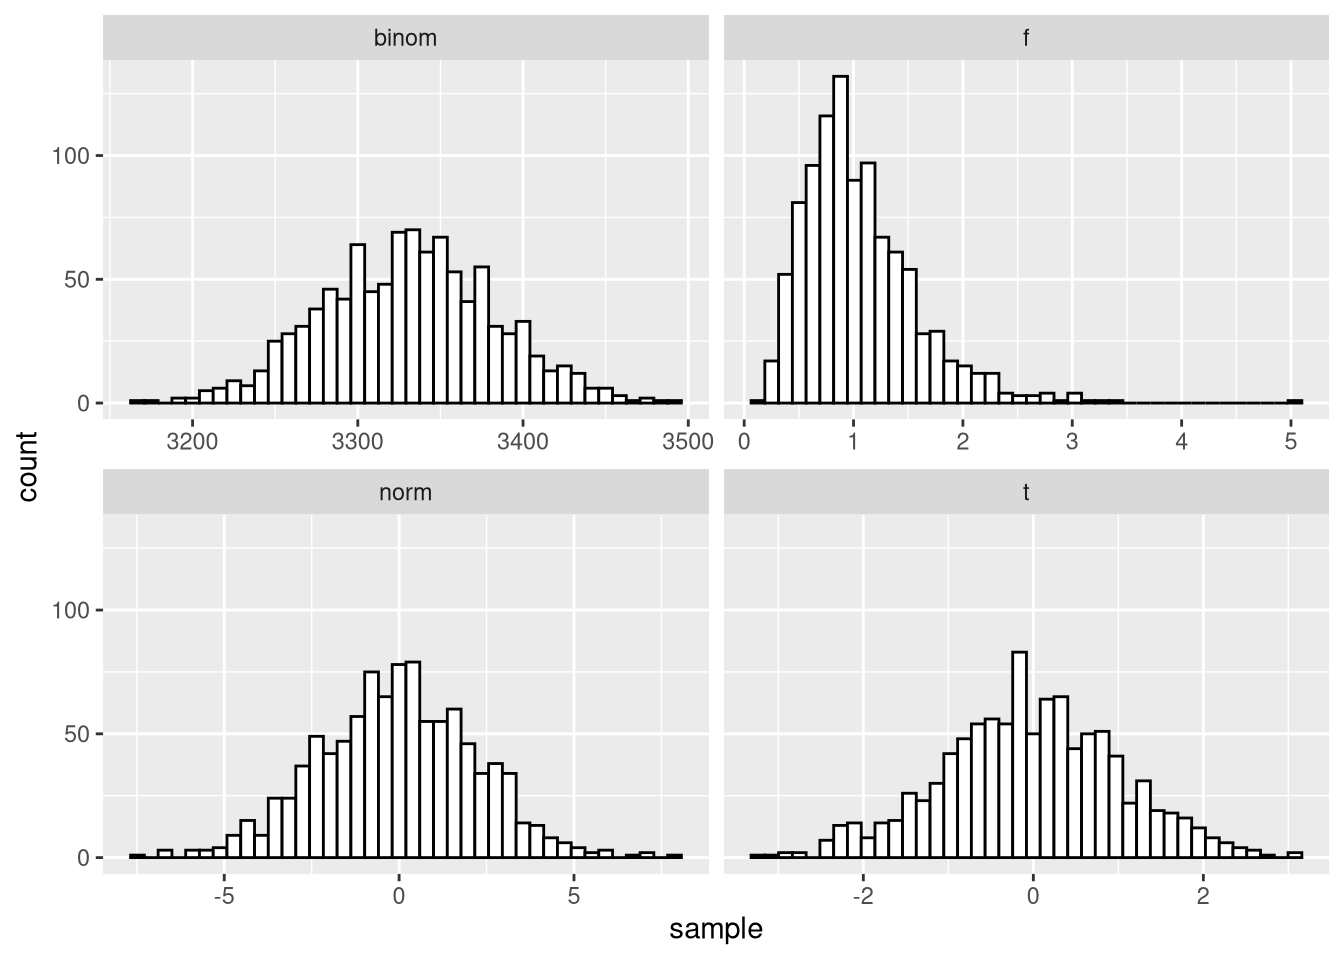
\includegraphics{Robustheit-und-Voraussetzungstests_files/figure-latex/unnamed-chunk-35-1.pdf}

\hypertarget{aufgabe-3}{%
\subsection{Aufgabe}\label{aufgabe-3}}

Erstelle eine Funktion \texttt{gen\_distributed\_values}, die mit Hilfe von \texttt{if}-Statements anhand eines Arguments \texttt{distribution} und eines Arguments \texttt{n} einen Vektor an Zufallszahlen generiert. Dabei soll \texttt{distribution} angeben, welche aus drei möglichen Verteilungen genutzt wird. Denke außerdem an mögliche Verteilungseigenschaften der genutzten Funktionen und füge sie als optionale Argumente zur Funktion hinzu.

Antwort

\begin{Shaded}
\begin{Highlighting}[]
\NormalTok{gen\_distributed\_values }\OtherTok{\textless{}{-}} \ControlFlowTok{function}\NormalTok{(distribution,}
\NormalTok{                                   n,}
                                   \AttributeTok{df =} \DecValTok{1}\NormalTok{,}
                                   \AttributeTok{lambda =} \DecValTok{25}\NormalTok{,}
                                   \AttributeTok{rate =} \DecValTok{5}\NormalTok{) \{}
  \ControlFlowTok{if}\NormalTok{(distribution }\SpecialCharTok{==} \StringTok{\textquotesingle{}t\textquotesingle{}}\NormalTok{)\{}
    \FunctionTok{return}\NormalTok{(}\FunctionTok{rt}\NormalTok{(n, df))}
\NormalTok{  \}}\ControlFlowTok{else} \ControlFlowTok{if}\NormalTok{(distribution }\SpecialCharTok{==} \StringTok{\textquotesingle{}pois\textquotesingle{}}\NormalTok{)\{}
    \FunctionTok{return}\NormalTok{(}\FunctionTok{rpois}\NormalTok{(n, lambda))}
\NormalTok{  \}}\ControlFlowTok{else} \ControlFlowTok{if}\NormalTok{(distribution }\SpecialCharTok{==} \StringTok{\textquotesingle{}exp\textquotesingle{}}\NormalTok{)\{}
    \FunctionTok{return}\NormalTok{(}\FunctionTok{rexp}\NormalTok{(n, rate))}
\NormalTok{  \}}
  \FunctionTok{print}\NormalTok{(}\StringTok{\textquotesingle{}Distribution is not implemented, returning zeros\textquotesingle{}}\NormalTok{)}
  \FunctionTok{return}\NormalTok{(}\FunctionTok{numeric}\NormalTok{(n))}
\NormalTok{\}}

\FunctionTok{gen\_distributed\_values}\NormalTok{(}\StringTok{\textquotesingle{}pois\textquotesingle{}}\NormalTok{,}
                       \DecValTok{5}\NormalTok{,}
                       \AttributeTok{lambda =} \DecValTok{3}\NormalTok{)}
\end{Highlighting}
\end{Shaded}

\begin{verbatim}
## [1] 4 4 3 5 2
\end{verbatim}

\hypertarget{schleifen}{%
\section{Schleifen}\label{schleifen}}

Bei so gut wie allen Simulationsproblemen stehen wir vor der Situation, dass wir eine Operation, zum Beispiel das Generieren einer gewissen Zahl an Zufallswerten und die Berechnung der zugehörigen Teststatistik, mehrere hundert Mal ausführen wollen.

Wir könnten jetzt die Operation mehrere hundert mal in unser Skript schreiben, damit würden wir aber zum Einen Fehler einladen, zum Anderen viel zu viel Lebenszeit verschwenden.

Deswegen gibt es in so gut wie jeder Programmiersprache irgendeine Form von Ausdrücken, die eine \emph{iterative} Wiederholung eines Ausdrucks ermöglichen.

Ein Beispiel für die Anweisung einer solchen iterativen Wiederholung sind Schleifen.
In R gibt es davon drei Arten:

\begin{itemize}
\item
  \texttt{repeat} - die flexibelste Schleife, die so lange wiederholt bis sie mit \texttt{break} unterbrochen wird
\item
  \texttt{while} - eine Schleife, die zu Beginn jeder Wiederholung einen logischen Test durchführt und bei Zutreffen die Operation wiederholt
\item
  \texttt{for} - die unflexibelste der drei Möglichkeiten. \texttt{for} iteriert einen Wert durch einen Vektor oder eine Liste, bis alle Einträge einmal dran waren. Das heißt, dass wir eine feste Laufzeit und damit den einfachsten Umgang haben, weswegen wir auch \texttt{for} in diesem Kurs verwenden werden.
\end{itemize}

Die \texttt{for}-Syntax sieht dabei wie folgt aus:

\begin{Shaded}
\begin{Highlighting}[]
\ControlFlowTok{for}\NormalTok{(value }\ControlFlowTok{in}\NormalTok{ vector)\{}
\NormalTok{  do something}
\NormalTok{\}}
\end{Highlighting}
\end{Shaded}

Um jetzt Beispielsweise alle Werte von eins bis zehn durch zu laufen und jeden Wert auszugeben können wir den folgenden Ausdruck benutzen:

\begin{Shaded}
\begin{Highlighting}[]
\ControlFlowTok{for}\NormalTok{(i }\ControlFlowTok{in} \FunctionTok{seq\_len}\NormalTok{(}\DecValTok{10}\NormalTok{))\{}
  \FunctionTok{print}\NormalTok{(i)}
\NormalTok{\}}
\end{Highlighting}
\end{Shaded}

\begin{verbatim}
## [1] 1
## [1] 2
## [1] 3
## [1] 4
## [1] 5
## [1] 6
## [1] 7
## [1] 8
## [1] 9
## [1] 10
\end{verbatim}

Wie man an diesem Beispiel schon sehen kann, können wir in der Schleife auf den \texttt{i}-Wert zugreifen. Das können wir zum Beispiel benutzen, um die ersten zehn Zahlen der Fibonacci-Reihe zu berechnen, in der jeder Wert die Summe der zwei vorhergegangenen ist:

\begin{Shaded}
\begin{Highlighting}[]
\NormalTok{fib }\OtherTok{\textless{}{-}} \FunctionTok{numeric}\NormalTok{(}\DecValTok{10}\NormalTok{)}
\ControlFlowTok{for}\NormalTok{(i }\ControlFlowTok{in} \FunctionTok{seq\_along}\NormalTok{(fib))\{}
  \ControlFlowTok{if}\NormalTok{(i}\SpecialCharTok{\textless{}}\DecValTok{3}\NormalTok{)\{ }\CommentTok{\# die ersten zwei Stellen müssen Einsen sein}
\NormalTok{    fib[i] }\OtherTok{\textless{}{-}} \DecValTok{1}
\NormalTok{  \}}\ControlFlowTok{else}\NormalTok{\{}
\NormalTok{    fib[i] }\OtherTok{\textless{}{-}}\NormalTok{ fib[i}\DecValTok{{-}1}\NormalTok{] }\SpecialCharTok{+}\NormalTok{ fib[i}\DecValTok{{-}2}\NormalTok{] }\CommentTok{\# nimm die letzten zwei Einträge und summier sie auf}
\NormalTok{  \}}
\NormalTok{\}}
\NormalTok{fib}
\end{Highlighting}
\end{Shaded}

\begin{verbatim}
##  [1]  1  1  2  3  5  8 13 21 34 55
\end{verbatim}

In diesem Beispiel ist noch ein weiteres Programmier-Prinzip sichtbar, die \emph{Allokation} des Ergebnis-Vektors vor der Berechnung der Werte. Damit ist einfach gemeint, dass wir den leeren \texttt{fib}-Vektor erstellt haben, bevor wir mit der Schleife angefangen haben.

Der Grund für dieses Vorgehen ist, dass jedes Anlegen eines Vektors einer bestimtmen Größe ein bisschen Rechenzeit kostet. Wenn wir von vornherein festlegen, wie lang der Vektor werden soll, müssen wir nur einen Vektor anlegen. Wenn wir stattdessen wie im folgenden Beispiel in jeder Iteration den Vektor vergrößern, erstellt R implizit in jeder Iteration einen neuen Vektor.

\begin{Shaded}
\begin{Highlighting}[]
\NormalTok{fib }\OtherTok{\textless{}{-}} \DecValTok{1}
\ControlFlowTok{for}\NormalTok{(i }\ControlFlowTok{in} \FunctionTok{seq\_len}\NormalTok{(}\DecValTok{10}\NormalTok{))\{}
  \ControlFlowTok{if}\NormalTok{(i}\SpecialCharTok{\textless{}}\DecValTok{3}\NormalTok{)\{ }
\NormalTok{    fib[i] }\OtherTok{\textless{}{-}} \DecValTok{1}
\NormalTok{  \}}\ControlFlowTok{else}\NormalTok{\{}
\NormalTok{    fib[i] }\OtherTok{\textless{}{-}}\NormalTok{ fib[i}\DecValTok{{-}1}\NormalTok{] }\SpecialCharTok{+}\NormalTok{ fib[i}\DecValTok{{-}2}\NormalTok{] }
\NormalTok{  \}}
\NormalTok{\}}
\NormalTok{fib}
\end{Highlighting}
\end{Shaded}

\begin{verbatim}
##  [1]  1  1  2  3  5  8 13 21 34 55
\end{verbatim}

Bei 10 Stellen ist der Unterschied noch nicht wirklich bemerkbar. Wenn wir jetzt aber das ganze in Funktionen verpacken und für längere Sequenzen laufen lassen und die Laufzeit stoppen sehen wir den Unterschied:

\begin{Shaded}
\begin{Highlighting}[]
\NormalTok{fib\_alloc }\OtherTok{\textless{}{-}} \ControlFlowTok{function}\NormalTok{(n)\{}
\NormalTok{  fib }\OtherTok{\textless{}{-}} \FunctionTok{numeric}\NormalTok{(n)}
  \ControlFlowTok{for}\NormalTok{(i }\ControlFlowTok{in} \FunctionTok{seq\_along}\NormalTok{(fib))\{}
    \ControlFlowTok{if}\NormalTok{(i}\SpecialCharTok{\textless{}}\DecValTok{3}\NormalTok{)\{ }
\NormalTok{      fib[i] }\OtherTok{\textless{}{-}} \DecValTok{1}
\NormalTok{    \}}\ControlFlowTok{else}\NormalTok{\{}
\NormalTok{      fib[i] }\OtherTok{\textless{}{-}}\NormalTok{ fib[i}\DecValTok{{-}1}\NormalTok{] }\SpecialCharTok{+}\NormalTok{ fib[i}\DecValTok{{-}2}\NormalTok{] }
\NormalTok{    \}}
\NormalTok{  \}}
  \FunctionTok{return}\NormalTok{(fib)}
\NormalTok{\}}


\NormalTok{fib\_no\_alloc }\OtherTok{\textless{}{-}} \ControlFlowTok{function}\NormalTok{(n)\{}
\NormalTok{  fib }\OtherTok{\textless{}{-}} \DecValTok{1}
  \ControlFlowTok{for}\NormalTok{(i }\ControlFlowTok{in} \FunctionTok{seq\_len}\NormalTok{(n))\{}
    \ControlFlowTok{if}\NormalTok{(i}\SpecialCharTok{\textless{}}\DecValTok{3}\NormalTok{)\{ }
\NormalTok{      fib[i] }\OtherTok{\textless{}{-}} \DecValTok{1}
\NormalTok{    \}}\ControlFlowTok{else}\NormalTok{\{}
\NormalTok{      fib[i] }\OtherTok{\textless{}{-}}\NormalTok{ fib[i}\DecValTok{{-}1}\NormalTok{] }\SpecialCharTok{+}\NormalTok{ fib[i}\DecValTok{{-}2}\NormalTok{] }
\NormalTok{    \}}
\NormalTok{  \}}
  \FunctionTok{return}\NormalTok{(fib)}
\NormalTok{\}}
\NormalTok{start }\OtherTok{\textless{}{-}} \FunctionTok{Sys.time}\NormalTok{()}
\NormalTok{a }\OtherTok{\textless{}{-}} \FunctionTok{fib\_alloc}\NormalTok{(}\DecValTok{100000}\NormalTok{)}
\NormalTok{runtime\_alloc }\OtherTok{\textless{}{-}} \FunctionTok{Sys.time}\NormalTok{() }\SpecialCharTok{{-}}\NormalTok{ start}
\NormalTok{start }\OtherTok{\textless{}{-}} \FunctionTok{Sys.time}\NormalTok{()}
\NormalTok{b }\OtherTok{\textless{}{-}} \FunctionTok{fib\_no\_alloc}\NormalTok{(}\DecValTok{100000}\NormalTok{)}
\NormalTok{runtime\_no\_alloc }\OtherTok{\textless{}{-}} \FunctionTok{Sys.time}\NormalTok{() }\SpecialCharTok{{-}}\NormalTok{ start}

\NormalTok{runtime\_alloc}
\end{Highlighting}
\end{Shaded}

\begin{verbatim}
## Time difference of 0.03389716 secs
\end{verbatim}

\begin{Shaded}
\begin{Highlighting}[]
\NormalTok{runtime\_no\_alloc}
\end{Highlighting}
\end{Shaded}

\begin{verbatim}
## Time difference of 0.0829339 secs
\end{verbatim}

Mehr als die Hälfte der Zeit geht für das Erstellen des neuen Vektors drauf!

\hypertarget{aufgabe-4}{%
\subsection{Aufgabe}\label{aufgabe-4}}

In QM-2 habt Ihr im Rahmen des zentralen Grenzwertsatzes gelernt, dass die Verteilungsfunktion der z-Transformation der n-ten Summe einer Reihe von unabhängigen Zufallsvariablen für wachsendes n schwach gegen die Standardnormalverteilung konvergiert.

Schreibe eine Funktion, die für eine gegebene Anzahl an Summen und eine gegebene Verteilungsklasse (und den entsprechenden Parametern inklusive der Stichprobengröße) einen Vektor mit den entsprechenden Summen zurückgibt.
Nutze dafür deine Funktion aus der letzten Aufgabe.

Nutze diese Funktion dann um ein Histogramm mit 5000 dieser z-transformierten Summen zu erstellen.

Antwort

\begin{Shaded}
\begin{Highlighting}[]
\NormalTok{gen\_central\_lim\_vec }\OtherTok{\textless{}{-}} \ControlFlowTok{function}\NormalTok{(N, }
\NormalTok{                                distribution,}
\NormalTok{                                n,}
                                \AttributeTok{df =} \DecValTok{1}\NormalTok{,}
                                \AttributeTok{lambda =} \DecValTok{25}\NormalTok{,}
                                \AttributeTok{rate =} \DecValTok{5}\NormalTok{) \{}
  
\NormalTok{  ret\_vec }\OtherTok{\textless{}{-}} \FunctionTok{numeric}\NormalTok{(N)}
  \ControlFlowTok{for}\NormalTok{(i }\ControlFlowTok{in} \FunctionTok{seq\_len}\NormalTok{(N))\{}
\NormalTok{    ret\_vec[i] }\OtherTok{\textless{}{-}} \FunctionTok{sum}\NormalTok{(}\FunctionTok{gen\_distributed\_values}\NormalTok{(distribution,}
\NormalTok{                                      n,}
\NormalTok{                                      df,}
\NormalTok{                                      lambda,}
\NormalTok{                                      rate))}
\NormalTok{  \}}
  \FunctionTok{return}\NormalTok{(ret\_vec)}
\NormalTok{\}}

\FunctionTok{tibble}\NormalTok{(}\AttributeTok{sample =} \FunctionTok{scale}\NormalTok{(}\FunctionTok{gen\_central\_lim\_vec}\NormalTok{(}\DecValTok{5000}\NormalTok{, }\StringTok{\textquotesingle{}exp\textquotesingle{}}\NormalTok{, }\DecValTok{1000}\NormalTok{,}\AttributeTok{rate =} \DecValTok{5}\NormalTok{))) }\SpecialCharTok{\%\textgreater{}\%} 
  \FunctionTok{ggplot}\NormalTok{(}\FunctionTok{aes}\NormalTok{(}\AttributeTok{x =}\NormalTok{ sample)) }\SpecialCharTok{+}
  \FunctionTok{geom\_histogram}\NormalTok{(}\AttributeTok{binwidth =}\NormalTok{ .}\DecValTok{1}\NormalTok{,}
                 \AttributeTok{color =} \StringTok{\textquotesingle{}grey\textquotesingle{}}\NormalTok{,}
                 \AttributeTok{fill =} \StringTok{\textquotesingle{}white\textquotesingle{}}\NormalTok{)}
\end{Highlighting}
\end{Shaded}

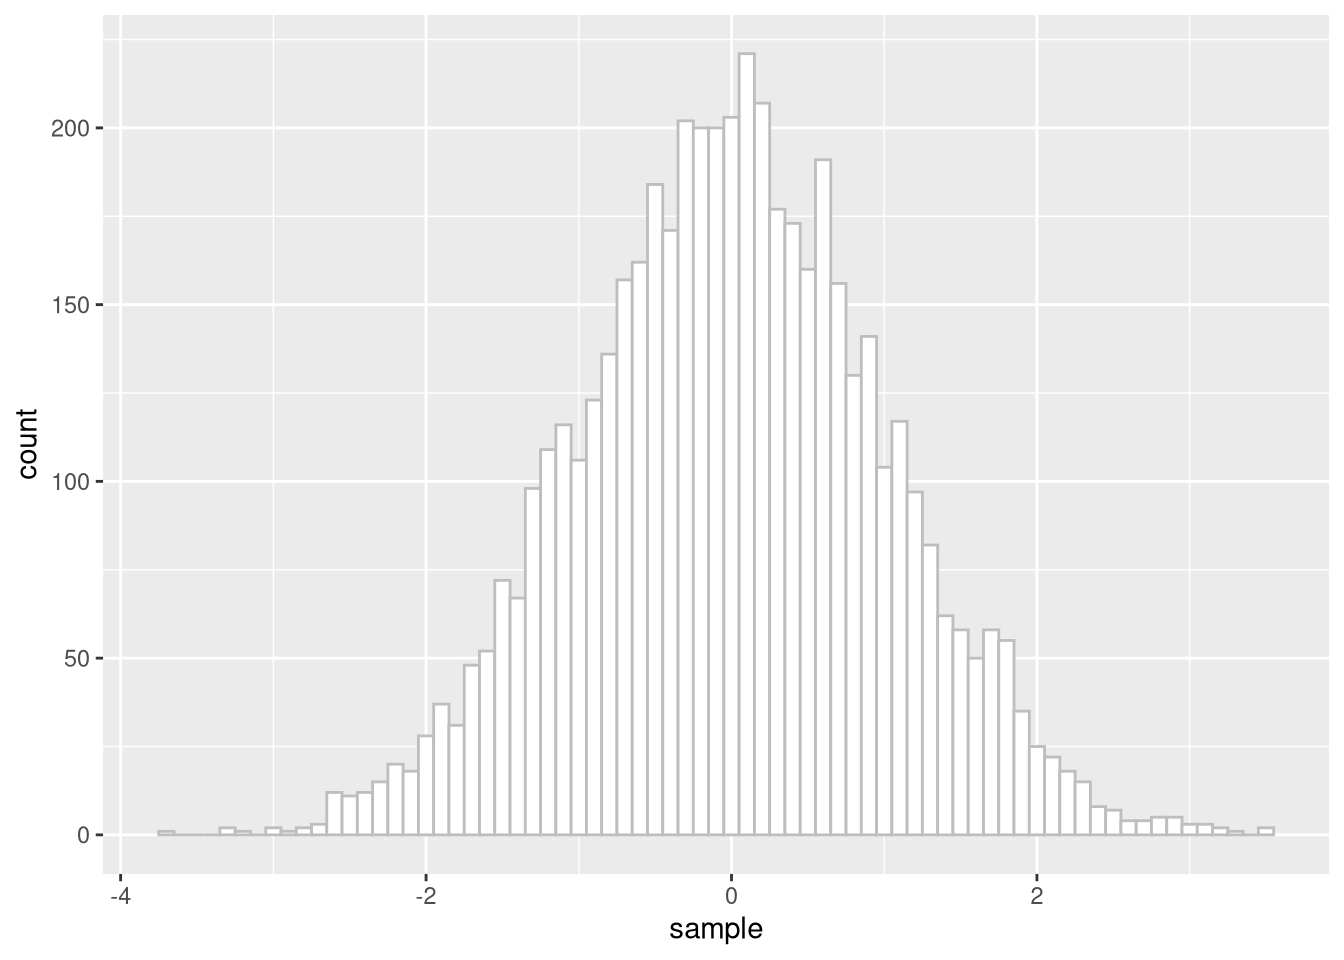
\includegraphics{Robustheit-und-Voraussetzungstests_files/figure-latex/unnamed-chunk-42-1.pdf}

  \bibliography{book.bib}

\end{document}
